\section {ОРГАНИЗАЦИОННО-ЭКОНОМИЧЕСКИЙ РАЗДЕЛ}
\subsection {Планирование разработки программного продукта с построением графика}
В дипломном проекте производится «Разработка программного модуля анализа защищённости СВТ от ВПО». В данном разделе определяется трудоемкость и затраты на создание ПО, а также производится расчет времени, необходимого для создания базы знаний, необходимой для работы программного средства в рамках испытания. 
\subsubsection {Определение трудоемкости и продолжительности работ по разработке программного модуля анализа защищённости СВТ от ВПО.}
Процесс разработки включает: обзор и анализ программных средств схожей тематики, анализ и выбор программных продуктов для создания программы; отладка; испытание. В свою очередь каждый из этих этапов можно подразделить на отдельные подэтапы.
Согласно ГОСТ 23501.1-79 регламентируются следующие стадии проведения исследования:
\begin {itemize}
	\item техническое задание – ТЗ (ГОСТ 23501.2-79);
	\item эскизный проект – ЭП (ГОСТ 23501.5-80);
	\item технический проект – ТП (ГОСТ 23501.6-80);
	\item рабочий проект – РП (ГОСТ 23501.11-81);
	\item внедрение – ВП (ГОСТ 23501.15-81).
\end {itemize}

Планирование стадий и содержания работ осуществляется в соответствии с \cite {ECONOMICS}. На всех стадиях проведения исследования выполняются следующие виды работ, перечень которых показан в таблице \ref {table:joblist}.

\begin{table}
	\begin {tabular}{|p{10em}|p{20em}|}
	\hline
	Стадии разработки & Перечень работ \\ \hline
	Техническое задание & -- постановка задачи; \\
	&  -- подбор литературы; \\
	& -- сбор исходных данных; \\
	& -- определение требований к системе; \\
	& -- определение стадий, этапов и сроков разработки ПО;\\ \hline
	Эскизный проект & -- анализ программных средств схожей тематики; \\
	&  -- разработка общей структуры ПО; \\
	& -- разработка структуры программы по подсистемам; \\
	& -- документирование; \\ \hline
	Технический проект & -- определение требований к ПО; \\
	&  -- выбор инструментальных средств; \\
	& -- определение свойств и требований к аппаратному обеспечению; \\ \hline
	Рабочий проект & -- верстка и дизайн; \\
	&  -- программирование; \\
	& -- тестирование и отладка ПО; \\
	& -- разработка программной документации; \\
	& -- согласование и утверждение работоспособности системы; \\ \hline
	Внедрение & -- опытная эксплуатация; \\
	&  -- программирование; \\
	& -- анализ данных, полученных в результате эксплуатации; \\
	& -- корректировка технической документации по результатам испытаний; \\ \hline
	\end {tabular}
	\caption{Перечень работ на каждой стадии проведения исследования}
	\label{table:joblist}
\end{table}

Трудоемкость выполнения работ по созданию ПО на каждой из стадий определяется в соответствии с \cite {ECONOMICSSECTION} и \cite {ECONOMICSDIPLOMA}.

Трудоемкость выполнения работ по созданию ПО определяется по сумме трудоемкости этапов и видов работ, оцениваемых экспертным путем в человеко-днях, и носит вероятностный характер, так как зависит от множества трудно учитываемых факторов.

Трудоемкость каждого вида работ определяется по формуле \eqref {eq:worksize}.
\begin {equation}
    \label {eq:worksize}
    t_i = \frac {3 * t_{min} + 2 * t_{max}}{5},
\end {equation}
где:

$t_{min}$ – минимально возможная трудоемкость выполнения отдельного вида работ;

$t_{max}$ – максимально возможная трудоемкость выполнения отдельного вида работ.

Продолжительность каждого вида работ в календарных днях ($T_i$) определяется по формуле \eqref {eq:calendarwork}, в днях:
\begin {equation}
    \label {eq:calendarwork}
    T_i = \frac {t_i}{\text{Ч}_i} * K_{\textup{вых}},
\end {equation}
где:

$t_i$ – трудоемкость работ, человек-дней;

$\text{Ч}_i$ – численность исполнителей, человек;

$K_{\textup{вых}}$ – коэффициент, учитывающий выходные и праздничные дни:
\begin {equation*}
    K_{\textup{вых}} = \frac {K_{\textup{кал.}}}{K_{\textup{раб.}}},
\end {equation*}	 
где:

$K_{\textup{кал}}$ – число календарных дней;

$K_{\textup{раб.}}$ – рабочие дни;

$K_{\textup{вых}}=1,3$.

Полный список видов и этапов работ по созданию ПО, экспертные оценки и расчетные величины их трудоемкости, а также продолжительность каждого вида работ, рассчитанные по формулам \eqref{eq:worksize} и \eqref{eq:calendarwork}, представлены в таблице \ref {table:worklength}

\begin{longtable}{| p{2em}|>{\raggedright\arraybackslash}p{12em}|p{2em}|p{2em}|p{2em}|p{2em}|p{5em}|}
	\caption{Расчёт трудоёмкости и продолжительности работ по созданию ПО}\\ \hline
	\label{table:worklength}
	\rotatebox[origin=c]{90}{№ работы} & Стадии разработки & \multicolumn{3}{|p{6em}|}{\rotatebox[origin=c]{90}{Трудоёмкость, чел.дни}} & \rotatebox[origin=c]{90}{Количество работников} & \rotatebox[origin=c]{90}{\parbox{8em}{Продолжительность работ, \\ календарные дни}} \\ \cline{3-7}
	& & $t_{min}$ & $t_{max}$ & $t_i$ & $\text{Ч}_i$ & $T_i$  \endfirsthead 
	\multicolumn{7}{c}{{\tablename\ \thetable{} -- продолжение}} \\ \hline
	1 & 2 & 3 & 4 & 5 & 6 & 7\endhead\hline
	1 & 2 & 3 & 4 & 5 & 6 & 7\\ \hline
	\multicolumn{7}{|c|}{Техническое задание} \\ \hline
	1 & - постановка задачи & 2 & 2 & 2 & 1 & 2.6 \\ \hline
	2 & - подбор литературы & 4 & 7 & 5.2 & 1 & 6.8 \\ \hline
	3 & - сбор исходных данных & 8 & 12 & 9.6 & 1 & 12.5\\ \hline
	4 & - определение требований к системе & 1 & 2 & 1.4 & 1 & 1.8\\ \hline
	5 & - определение стадий, этапов и сроков разработки ПО & 2 & 3 & 2.4 & 1 & 3.1\\ \hline
	\multicolumn{7}{|c|}{Эскизный проект}\\ \hline
	6 & - анализ программных средств схожей тематики & 7 & 8 & 7.4 & 1 & 9.6\\ \hline
	7 & - разработка общей структуры ПО & 3 & 5 & 3.8 & 1 & 4.9\\ \hline
	8 & - разработка структуры программы по подсистемам & 4 & 6 & 4.8 & 1 & 	6.2\\ \hline
	9 & - документирование & 1 & 3 & 1.8 & 1 & 2.3\\ \hline
	\multicolumn{7}{|c|}{Технический проект}\\ \hline
	10 & - определение требований к ПО	& 1 & 2 & 1.4 & 1 & 1.8\\ \hline
	11 & - выбор инструментальных средств & 1 & 1 & 1 & 1 & 1,3\\ \hline
	12 & - определение свойств и требований  к аппаратному обеспечению & 1 & 1 & 1 & 1 & 1.3\\ \hline
	\multicolumn{7}{|c|}{Рабочий проект}\\ \hline
	13 & - дизайн проекта & 2 & 4 & 2.8 & 1 & 3.6\\ \hline
	14 & - программирование & 8 & 12 & 9.6 & 1 & 12.5\\ \hline
	15 & - тестирование и отладка ПО & 20 & 25 & 22 & 1 & 28.6\\ \hline
	16 & - разработка программной документации & 3 & 5 & 4.8 & 1 & 6.2\\ \hline
	17 & - согласование и утверждение работоспособности системы & 2 & 3 & 2.4 & 1 & 3.1\\ \hline
	\multicolumn{7}{|c|}{Внедрение}\\ \hline
	18 & - опытная эксплуатация & 11 & 22 & 15.4 & 1 & 20\\ \hline
	19 & - анализ данных, полученных в результате эксплуатации & 3 & 4 & 3.4 & 1 & 4.4\\ \hline
	20 & - корректировка технической документации по результатам испытаний & 1 & 2 & 1.4 & 1 & 1.8\\ \hline
	& \textbf{Общая трудоёмкость разработки} & & & \textbf{104} & & \textbf{134}\\ \hline
\end{longtable}
Таким образом, общая продолжительность проведения работ составит 134 календарных дней.

\subsubsection {Построение ленточного графика проведения исследования}
В качестве инструмента планирования работ используем ленточный график. Ленточный график позволяет наглядно представить логическую последовательность и взаимосвязь отдельных работ, срок начала и срок окончания работ. Он представляет собой таблицу, где перечислены наименования стадий разработки и видов работ, длительность выполнения каждого вида работ. Продолжением таблицы является график, отражающий продолжительность каждого вида работ в виде отрезков времени, которые располагаются в соответствии с последовательностью выполнения работ. 

Ленточный график разработки ПО, построенный по данным таблицы \ref {table:worklength}, приведен на рисунке \ref {fig:workflow}.

\begin {figure}
	\centering
	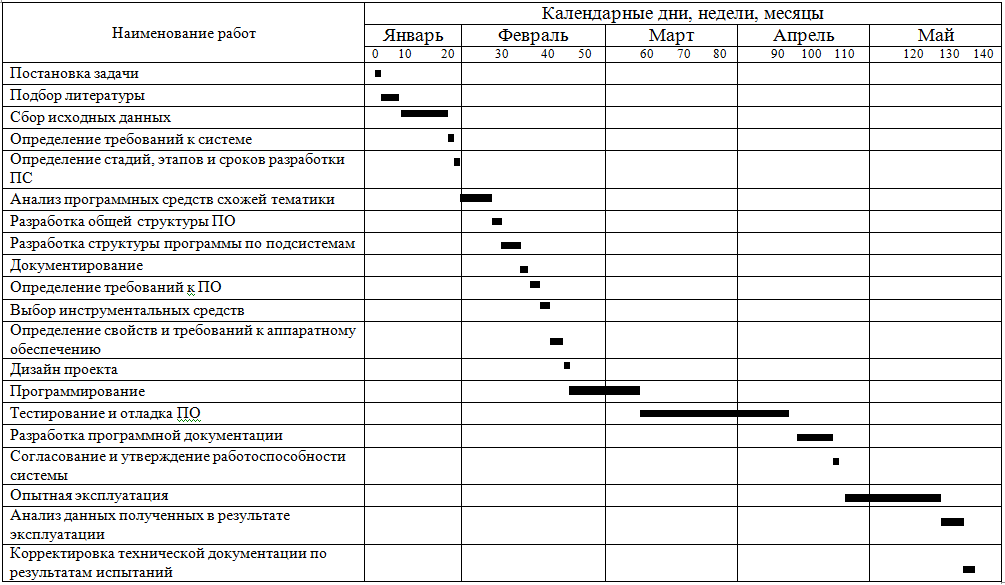
\includegraphics[angle=90,scale=0.95]{img/WorkFlow.png}
	\caption{Ленточный график разработки ПО}
	\label{fig:workflow}
\end {figure}

\subsection {Расчёт сметы затрат на разработку программного продукта}

Сметная стоимость проектирования и внедрения программы включает в себя следующие затраты, определяемые по формуле \eqref{eq:project}:
\begin {equation}
    \label {eq:project}
    C_{\textup{пр}}=C_{\textup{осн}} + C_{\textup{доп}} + C_{\textup{соц}} + C_{\textup{м}} + C_{\textup{маш}},
\end {equation}

где

$C_{\textup{пр}}$ – стоимость разработки ПО;

$C_{\textup{осн}}$ – основная заработная плата исполнителей;

$C_{\textup{доп}}$ – дополнительная заработная плата исполнителей, учитывающая потери времени на отпуска и болезни (принимается в среднем 10\% от основной заработной платы);

$C_{\textup{соц}}$ – отчисления во внебюджетные фонды государственного социального страхования (пенсионный фонд, фонд обязательного медицинского страхования, фонд социального страхования), рассчитываются как 30,2\% от основной и дополнительной заработной платы;

$C_{\textup{м}}$ – затраты на используемые материалы;

$C_{\textup{маш.вр}}$ – стоимость машинного времени.

$C_{\textup{н}}$ – накладные расходы включают затраты на управление, уборку, ремонт, электроэнергию, отопление и др. (принимаются в размере 60\% от основной и дополнительной заработной платы);

\begin {center}
	\textbf{Основная заработная плата исполнителей.}
\end {center}

На статью «Заработная плата» относят заработную плату научных, инженерно-технических и других работников, непосредственно участвующих в разработке ПО. Расчет ведётся по формуле \eqref {eq:executer_salary}:
\begin {equation}
    \label{eq:executer_salary}
    \text{З}_{\textup{исп}} = \text{З}_{\textup{ср}} *\text{Т},
\end {equation}

где

$\text{З}_{\textup{исп}}$ – заработная плата исполнителей (руб.);

$\text{З}_{\textup{ср}}$ – средняя тарифная ставка работника организации разработчика ПО (руб./чел./дни);

$\text{Т}$ – трудоемкость разработки ПО (чел.дни).

$\text{З}_{\textup{ср}}$ определяется по формуле \eqref {eq:average_salary}:
\begin {equation}
    \label {eq:average_salary}
    \text{З}_{\textup{ср}} = \text{С} / \text{Ф}_{\textup{мес}},
\end {equation}
где

$\text{С}$ – зарплата труда на текущий момент времени (руб./мес.);

$\text{Ф}_{\textup{мес}}$ – месячный фонд рабочего времени исполнителя (дни).

Затраты на статью «Заработной платы» приведены в таблице \ref{table:cost_salary}.

\begin{table}[h]
	\begin {tabular}{|p{2em}|p{6em}|p{4em}|p{6em}|p{7em}|p{6em}|}
		\hline
		№ & Исполнитель & Оклад, руб./мес. & Оклад., руб./день & Трудоемкость, чел.дни & Сумма, руб.\\ \hline
		1 & Инженер-программист & 60000 & 2000 & 104 & 208000 \\ \hline
		\multicolumn{4}{|p{16em}|}{Общая основная зарплата исполнителей, $C_{\textup{осн}}$} & 104 & 208000\\ \hline
	\end {tabular}
	\caption{Затраты на заработную плату}
	\label{table:cost_salary}
\end{table}

\begin {center}
	\textbf{Дополнительная заработная плата}
\end {center}

Дополнительная заработная плата на период разработки ПО рассчитывается относительно основной и составляет 10\% от ее величины:
\begin {equation}
                                  C_{\textup{доп}} = C_{\textup{осн}} * 0,1 = 20800 (\text{руб.})
\end {equation}

\begin {center}
	\textbf{Расчет отчислений на социальное страхование}
\end {center}

Социальное страхование включает отчисления во все внебюджетные фонды, в том числе пенсионный, занятости, обязательного медицинского страхования, социального страхования. Отчисления на социальное страхование рассчитываются относительно выплаченной заработной платы (суммы основной и дополнительной заработной платы). Составляют 30,2\%:
\begin {equation}
                          C_{\textup{соц}} = (C_{\textup{осн}} + C_{\textup{доп}}) * 0,302
\end {equation}
\begin {equation*}
	C_{\textup{соц}} = (208000 + 20800) * 0,302 = 69097.6 (\text{руб.})
\end {equation*}

\begin {center}
	\textbf{Расчет расходов на материалы}
\end {center}

На эту статью относят все затраты на магнитные носители данных, бумагу, для печатных устройств, канцтовары и др. Затраты по ним определяются по экспертным оценкам. Расчет расходов на материалы приведен в таблице \ref{table:cost_materials}.

\begin{table}
	\begin {tabular}{|p{3em}|p{10em}|p{8em}|p{8em}|}
		\hline
		№ & Материалы & Количество, штуки & Стоимость, рубли\\ \hline
		1 & Бумага писчая, листов & 1000 & 400 \\ \hline
		2 & Картридж для принтера, шт. & 1 & 900\\ \hline
		3 & HDD Seagate Constellation ES.3 ST3000NM0033 для виртуальных машин/архивов с ВПО & 1 & 10746\\ \hline
		\multicolumn{3}{|p{21em}|}{Общая стоимость материалов, $C_{\textup{м}}$} & 12046\\ \hline
	\end {tabular}
	\caption{Стоимость материалов}
	\label{table:cost_materials}
\end{table}

\begin {center}
	\textbf{Накладные расходы}
\end {center}

На статью «Накладные расходы» относят расходы, связанные с управлением и организацией работ. Накладные расходы рассчитываются относительно основной заработной платы. Величина накладных расходов принимается равной 60\% от основной зарплаты исполнителей. Формула расчёта \eqref{eq:overhead_cost}:
\begin {equation}
    \label {eq:overhead_cost}
    C_{\textup{н}} = C_{\textup{осн}} * \text{К}
\end {equation}
где

$C_{\textup{н}}$ – накладные расходы (руб.);

$C_{\textup{осн}}$ – основная заработная плата исполнителей (руб.);
$\text{К}$ – коэффициент учета накладных расходов ($\text{К} = 0,6$)
\begin {equation*}
    C_{\textup{н}} = 208000 * 0,6 = 124800 (\text{руб.})
\end {equation*}

\begin {center}
	\textbf{Расчет стоимости машинного времени}
\end {center}

Затраты на машинное время, необходимое для разработки ПО, расходы на приобретение и подготовку материалов научно-технической информации, расходы на использование средствами связи. Расчет затрат на машинное время осуществляется по формуле \eqref{eq:computer_time}:
\begin {equation}
    \label{eq:computer_time}
    C_{\textup{маш.вр}} = \text{К}_{\textup{маш.вр}} * \text{З}_{\textup{маш.вр}}
\end {equation}

где
$\text{К}_{\textup{маш.вр}}$ – тарифная стоимость одного часа машинного времени ($\text{К}_{\textup{маш.вр}}=50 \text{руб./ч.}$)

Тарифная стоимость 1 суток работы составляет:
\begin {equation*}
    C_{\textup{cуток}} = 24 * \text{К}_{\textup{маш.вр}} = 24 * 50 = 1200 (\text{руб.})
\end {equation*}

$\text{З}_{\textup{маш.вр}}$ – машинное время, используемое на проведение работ.

Необходимое количество машинного времени для реализации проекта по разработке программы рассчитывается по формуле \eqref {eq:impl_time}:
\begin {equation}
    \label {eq:impl_time}
    \text{З}_{\textup{маш.вр}} = t_i * T_{\textup{см}} * T_{\textup{ср.маш}},
\end {equation}

где

$t_i$ – трудоемкость работ, чел.дней;

$T_{\textup{см}}$ – продолжительность рабочей смены (при пятидневной рабочей неделе $T{\textup{см}} = 8 \text{ч.}$);

$T{\textup{ср.маш}}$ – средний коэффициент использования машинного времени ($T{\textup{ср.маш}} = 0,7$).

Тогда:
\begin {equation*}
    \text{З}_{\textup{маш.вр}} = 104 * 8 * 0,7 = 582 (\text{ч.})
\end {equation*}

Стоимость машинного времени составит:
\begin {equation*}
    C_{\textup{маш.вр}} = 50 * 582 = 29100 (\text{руб.})
\end {equation*}

Результаты расчета затрат на проектирование программного обеспечения сведены в таблице \ref{table:cost_outlay}.
\begin{table}[h]
	\begin {tabular}{|p{3em}|p{10em}|p{6em}|p{6em}|p{6em}|}
		\hline
		№ & Наименование статей & Обозначение & Сумма, руб. & В \% к итогу\\ \hline
		1 & 2 & 3 & 4 & 5 \\ \hline
		1 & Основная заработная плата & $C_{\textup{осн}}$ & 208000 & 44.84 \\ \hline
		2 & Дополнительная заработная плата & $C_{\textup{доп}}$ & 20800 & 4.48\\ \hline
		3 & Отчисления на социальные нужды & $C_{\textup{соц}}$ & 69097.6 & 14.9\\ \hline
		4 & Материалы & $C{\textup{мат}}$ & 12046 & 2.6\\ \hline
		5 & Стоимость машинного времени & $C{\textup{маш.вр.}}$ & 29100 & 6.27\\ \hline
		6 & Накладные расходы & $C{\textup{н}}$ & 124800 & 26.9\\ \hline
		\multicolumn{2}{|p{13em}|}{Итого:} & $C{\textup{пр}}$ & 463843.6 & 100\\ \hline
	\end {tabular}
	\caption{Смета затрат на разработку и внедрение программы}
	\label{table:cost_outlay}
\end{table}

Таким образом, себестоимость разработки составляет \textbf{463843.6} руб.

Данная программа может быть реализована на рынке. При расчетном количестве реализованных программ (n=100), оптовая цена программы ($\text{Ц}_{\textup{опт}}$) может быть рассчитана по формуле \eqref {eq:wholesale}:
\begin {equation}
    \label {eq:wholesale}
    \text{Ц}_{\textup{опт}} =  \frac{C_{\textup{пр}}}{n} + \text{П} ;
\end {equation}
где

$C{\textup{пр}}$ – себестоимость разработки программы;

П – прибыль, определяется по формуле \eqref {eq:gains}:
\begin {equation}
    \label {eq:gains}
    \text{П}_i = \text{Ур} * \frac{C_{\textup{пр}}}{n} * 100,
\end {equation}
где

$\text{Ур}$ – средний уровень рентабельности ($\text{Ур} = 20\%$).

Таким образом, оптовая цена программы составит:
\begin {equation*}
\text{Ц}_{\textup{опт}} = 463843.6/100 + (463843.6/100)*0.2 = \textbf{5566.1} (\text{руб.})
\end {equation*}
Отпускная цена реализации программы потребителям (Цотп), рассчитывается по формуле \eqref {eq:saleprice}:
\begin {equation}
    \label {eq:saleprice}
    \text{Ц}_{\textup{отп}} = \text{Ц}_{\textup{опт}} + \text{НДС},
\end {equation}
где

НДС – налог на добавленную стоимость, рассчитывается в соответствии с действующей ставкой этого налога – 18\% от оптовой цены программы.
\begin {equation*}
    \text{Ц}_{\textup{отп}}  = 5566.1 + 5566.1*0.18 = 5566.1 + 1001,9 = \textbf{6568} (\text{руб.})
\end {equation*}

Таким образом, отпускная цена программы составит \textbf{6568}  руб., в том числе НДС – \textbf{1001,9}  руб.

\subsection {Расчёт основных технико-экономических показателей и эффективности использования программного продукта}
В настоящей дипломной работе проведена программная реализация алгоритмов, направленных на обнаружение похожего поведения вредоносного ПО, а также собран один из вариантов сред, используемых для исследования их поведения. При увеличении машинного времени, выделяемого для сбора цепочек на известных образцах ВПО, точность обнаружения потенциально неизвестных вирусов будет увеличена (т.к. скорость прогона образцов на данном хосте за сутки составляет около 6000 шт./сутки, за каждые $C_{\textup{cуток}} = 1200 \text{руб.}$ возможно  увеличение числа собранных цепочке на соответствующее число). 

Также предусматривается возможность доработки программного продукта в рамках использования других сред виртуализации. Это приведёт  к более эффективному использованию аппаратного обеспечения, на котором собираются цепочки вызовов ВПО на предоставляемых программе образцах, и, возможно, позволит увеличить число параллельно работающих виртуальных машин. Всё это предоставляет возможности для обнаружения новых вредоносных программ, имеющих подозрительное поведение.

\begin{longtable}{| >{\centering\arraybackslash}p{10em}|>{\centering\arraybackslash}p{6em}|>{\centering\arraybackslash}p{12em}|}
	\caption{Основные технико-экономические показатели проекта}\\ \hline
	\label{table:project_tth}
	Наименование показателя & Ед. измерения & Проектный вариант\endfirsthead
	\multicolumn{3}{c}{{\tablename\ \thetable{} -- продолжение}} \\ \hline
	1 & 2 & 3\endhead \hline
	1 & 2 & 3\\ \hline
	Способ обработки информации& --- & С применением ЭВМ и програмных средств \\ \hline
           Характеристики исследования: & & \\ \hline
	Язык программирования & --- & CPython 3.4\\ \hline
	Использованные технические средства: & &\\ \hline
	Хост для запуска виртуальных машин & --- & Intel Xeon E3-1245v3, 4 x 8Gb DDR1600, HDD 3 Tb/7200/64Mb, int. Video, LAN, ATX 1000W\\ \hline
	Принтер & --- & HP LaserJet 6L\\ \hline
	Количество исследователей & чел & 1\\ \hline
	Продолжительность проведения исследования & календарных дней & 134\\ \hline
	Трудоёмкость проведения исследования & чел-дней & 104\\ \hline
	Затраты на проведение исследования & руб. & 463843.6\\ \hline
	в том числе: &  & \\ \hline
	Стоимость расходных материалов & руб. & 12046\\ \hline
	Основная заработная плата & руб. & 208000\\ \hline
	Дополнительная заработная плата & руб. & 20800\\ \hline
	Отчисления на социальные нужды & руб. & 69097.6\\ \hline
	Накладные расходы & руб. & 124800\\ \hline
	Стоимость машинного времени & руб. & 29100\\ \hline
\end{longtable}

